\chapter[Ranking Computer Vision Service Issues using Emotion]
{Ranking Computer Vision Service Issues using Emotion\pubfootnote{Curumsing:2020semotion}}
\label{ch:semotion2020}
\graphicspath{{mainmatter/publications/figures/semotion2020/}}

\def\SEMNumPostsFromSO{1,425}	
\def\SEMNumPostsCategorised{1,825}	
\def\SEMNumPostsFromFiftyClassified{380}	
\def\SEMNumPostsFromFiftyNoise{70}	
\def\SEMNumPostsNoise{238}	\def\PctPostsNoise{13.04\%}
	
\def\SEMNumTaxACategorised{188}	\def\SEMPctTaxACategorised{10.30\%}
\def\SEMNumTaxBCategorised{1,579}	\def\SEMPctTaxBCategorised{86.52\%}
\def\SEMNumTaxAUnCategorised{1,410}	\def\SEMPctTaxAUnCategorised{77.26\%}
\def\SEMNumTaxBUnCategorised{19}	\def\SEMPctTaxBUnCategorised{1.04\%}
	
\def\SEMPctTaxACorrectness{22.87\%}
\def\SEMPctTaxACompleteness{47.87\%}
\def\SEMPctTaxADocumentation{23.94\%}
\def\SEMPctTaxBAPIUsage{22.29\%}	
\def\SEMPctTaxBDiscrepancy{16.34\%}	
\def\SEMPctTaxBErrors{32.05\%}	
\def\SEMPctTaxBReview{15.14\%}	
\def\SEMPctTaxBConceptual{11.02\%}	
\def\SEMPctTaxBAPIChange{1.08\%}	
\def\SEMPctTaxBLearning{2.09\%}	

\glsresetall
\begin{abstract}
Software developers are increasingly using \glslongpl{iws} to implement `intelligent' features. Studies show that incorporating \gls{ai} into an application increases technical debt, creates data dependencies, and introduces uncertainty due to non-deterministic behaviour. However, we know very little about the emotional state of software developers who deal with such issues. In this paper, we do a landscape analysis of emotion found in \SEMNumPostsFromSO{} \gls{so} posts about \glslongpl{cvs}. We investigate the application of an existing emotion classifier EmoTxt and manually verify our results. We found that the emotion profile varies for different question categories and that a new emotion schema is required to better represent the emotion present in \gls{so} questions. We propose an initial version of a new emotion classification scheme and confirm current findings that \gls{ai} is insufficient for automatic classification of emotion. 
\end{abstract}
\glsresetall

\section{Introduction}

Recent advances in artificial intelligence have provided software engineers with new opportunities to incorporate complex machine learning capabilities, such as computer vision, through cloud-based \glspl{iws}. These new set of services, typically offered as \glsac{api} calls are marketed as a way to reduce the complexity involved in integrating \glsac{ai}-components. However, recent work shows that software engineers struggle to use these \glspl{iws}~\citep{Cummaudo:2020icse}. 
%Furthermore, the accompanying documentation fails to address common issues experienced by software engineers and, often, engineers resort to online communication channels, such as, JIRA and Stack Overflow (\gls{so}) to seek advice from their peers~\citep{Cummaudo:2020icse}.

While seeking advice on the issues, software engineers tend to express their emotions (such as frustration or confusion) within the questions. Recognising the value of considering emotions, other researchers have investigated emotions expressed by software developers within communication channels~\citep{ortu2016} including \gls{so}~\citep{novielli2018, calefato2018}; the broad motivation of these works is to generally understand the emotional landscape and improve developer productivity~\citep{murgia2014, ortu2016, gachechiladze2017}. However, previous works have not directly focused on the nature of emotions expressed in questions related to \glspl{iws}. We also do not know if certain types of questions express stronger emotions.

The machine-learnt behaviour of these \glspl{iws} is typically non-deterministic and, given the dimensions of data used, their internal inference process is hard to reason about~\citep{Cummaudo:2019icsme}. Compounding the issue, documentation of these cloud systems does not explain the limits, nor how they were created (esp. data sets used to train them). This lack of transparency makes it difficult for even senior developers to properly reason about these systems, so their prior experience and anchors do not offer sufficient support~\citep{Cummaudo:2020icse}. In addition, adding machine learned behaviour to a system incurs ongoing maintenance concerns~\citep{Sculley2015}. There is a need to better understand emotions expressed by developers to inform cloud vendors and help them improve their documentation and error messages provided by their services.

This work builds on top of recent work that explored \textit{what} pain-points developers face when using \glspl{iws} through a general analysis of \SEMNumPostsFromSO{} \gls{so} posts (questions)~\citep{Cummaudo:2020icse} using an existing \gls{so} issue classification taxonomy~\citep{Beyer:2018fm}. In this work, we consider the emotional state expressed within these pain-points, using the same data set of \SEMNumPostsFromSO{} \gls{so} posts. We identify the emotions in each \gls{so} question, and investigate if the distribution of these emotions is similar across the various types of questions.

In order to classify emotions from \gls{so} posts, we use EmoTxt, a recently proposed toolkit for emotion recognition from text~\citep{novielli2018, calefato2017, calefato2018}. EmoTxt has been trained and built on \gls{so} posts using the emotion classification model proposed by~\citet{shaver1987}. The category of issue was manually determined in our prior work. 

% No one has classified emotion against problem types.
% Only previous work is EmoTxt who has looked @ emotion on \gls{so}.

The key findings of our study are:

%\todo{Anju: change findings}
\begin{itemize}
    \item The distribution of emotions is different across the taxonomy of issues.
    \item A deeper analysis of the results, obtained from the EmoTxt classifier, suggests that the classification model needs further refinement. Love and joy, the least expected emotions when discussing \glsac{api} issues, are visible across all categories.
    \item A different emotion classification scheme is required to better reflect the emotions within the questions.
\end{itemize}

In order to promote future research and permit replication, we make our data set publicly available.\footnote{See \url{http://bit.ly/2RiULgW}.} The paper structure is as follows: \cref{semotion2020:sec:EM} provides an overview on prior work surrounding the classification of emotions from text; \cref{semotion2020:sec:methodology} describes our research methodology;  \cref{semotion2020:sec:findings} presents the results from the EmoTxt classifier;  \cref{semotion2020:sec:discussion} provides a discussion of the results obtained; \cref{semotion2020:sec:implications} highlights the implications of our study; \cref{semotion2020:sec:threats} outlines the threats to validity; \cref{semotion2020:sec:conclusion} presents the concluding remarks.  


 
\section{Emotion Mining from Text}\label{semotion2020:sec:EM}

Several studies have investigated the role of emotions generally in software development~\citep{wrobel2013, Shaw:2003aa, ortu2016, gachechiladze2017}. Work in the area of behavioural software engineering established the link between software developer's happiness and productivity~\citep{Graziontin:2017}. Wrobel~\citep{wrobel2013} investigated the impact that software developers' emotion has on the development process and found that frustration and anger were amongst the emotions that posed the highest risk to developer's productivity.    

Recent studies focused on emotion mining from text within communication channels used by software engineers to communicate with their peers~\citep{murgia2014, ortu2016, gachechiladze2017, novielli2018}.~\citet{murgia2014} and~\citet{ortu2016} investigated the emotions expressed by developers within an issue tracking system, such as JIRA, by labelling issue comments and sentences written by developers using Parrott's framework.~\citet{gachechiladze2017} applied the Shaver framework to detect anger expressed in comments written by developers in JIRA. The Collab team~\citep{calefato2017, novielli2018} extended the work done by~\citet{ortu2016} and developed a gold standard data set collected from \gls{so} posts consisting of questions, comments and feedback. This data set was manually annotated using the Shaver's emotion model. The Shaver's model consists of a tree-structured, three level, hierarchical classification of emotions. The top level consists of six basic emotions namely, love, joy, anger, sadness, fear and surprise~\citep{shaver1987}. The subsequent levels further refines the granularity of the previous level. One of their recent work~\citep{novielli2018} involved 12 raters to manually annotate 4,800 posts (where each post included the question, answer and comments) from \gls{so}. The same question was assigned to three raters to reduce bias and subjectivity. Each coder was requested to indicate the presence/absence of each of the six basic emotions from the Shaver framework. As part of their work they developed an emotion mining toolkit, EmoTxt~\citep{calefato2017}. The work conducted by the Collab team is most relevant to our study since their focus is on identifying emotion from \gls{so} posts and their toolkit is trained on a large data set of \gls{so} posts.



\section{Methodology}\label{semotion2020:sec:methodology}

As mentioned in our introduction, this paper uses the data set reported in~\citeauthor{Cummaudo:2020icse}'s ICSE 2020 paper~\citep{Cummaudo:2020icse}. As this paper is in press, we reproduce a summary of the methodology used in constructing this data set methodology below. For full details, we refer to the original paper. Supplementary materials used for this work are provided for replication.\footnotemark[1]

Our research methodology consisted of the following steps: (i)~data extraction from \gls{so} resulting in 1,425 questions about intelligent \glspl{cvs}; (ii)~question classification using the taxonomy presented by \citet{Beyer:2018fm}; (iii)~automatic emotion classification using EmoTxt based on \citeauthor{shaver1987}'s emotion taxonomy \citep{shaver1987}; and (iv)~manual classification of 25 posts to better understand developers emotion. We calculated the inter-rater reliability between EmoTxt and our manually classified questions in two ways: (i)~to see the overall agreement between the three raters in applying the \citeauthor{shaver1987} emotions taxonomy, and (ii)~to see the overall agreement with EmoTxt's classifications. Further details are provided below.

\def \alexnumauthor {second}

\subsection{Data Set Extraction from \gls{so}}

\subsubsection{Intelligent Service Selection}

We contextualise this work within popular \gls{cvs} providers: Google Cloud~\citepweb{GoogleCloud:Home}, AWS~\citepweb{AWS:Home}, Azure~\citepweb{Azure:Home} and IBM Cloud~\citepweb{IBM:Home}.
We chose these four providers given their prominence and ubiquity as cloud service vendors, especially in enterprise applications~\citep{RightScaleInc:2018kJ}. We acknowledge other services beyond the four analysed which provide similar capabilities~\citepweb{Pixlab:Home,Clarifai:Home,Cloudsight:Home,DeepAI:Home,Imagaa:Home,Talkwaler:Home}. Additionally, only English-speaking services have been selected, excluding popular \glspl{cvs} from Asia (e.g.,~\citepweb{Megvii:Home,TupuTech:Home,YiTuTech:Home,SenseTime:Home,DeepGlint:Home}).

% \subsubsection{Defining a list of \glspl{iws}}
% There is no such global `list' of \glspl{iws} to search on. Therefore, we devised a \textit{corpus of initial terms} to help us with searching for terms on the Stack Exchange Data Explorer\footnote{\url{http://data.stackexchange.com/stackoverflow}} (SEDE). To start, we explored the various brands of these cloud services including their  permutations (e.g., \underline{G}oogle \underline{C}loud \underline{S}ervices and GCS) as well as various \gls{ai}-related products (e.g., Google Cloud \gls{ai}). This was achieved using extensive Google searches\footnote{This search was conducted on 17 January 2019}\def\footnotesearchdate{2} in addition to manually reviewing six `overview' pages for each platform. In total, 91 \glspl{iws} were found and were incorporated into our search terms\footnote{For reproducibility, this is available at \url{http://bit.ly/2ZcwNJO}.}.\def\footnotereproducability{3} 

% \subsubsection{Manual search for relevant, related terms} 
% We then ran a manual search\footnotemark[\footnotesearchdate{}] %Footnote RE 17 Jan 2019
% for each term to determine their relevancy. We achieved this by querying each term on the \gls{so} search feature and reviewed each result's question title and post previews for the first three pages of results. Additionally, we recorded user-defined \textit{Tags} of each post (up to five per question). We also reviewed similar tags (e.g., `project-oxford' for `azure-cognitive-services') and checked if each tag had synonyms (e.g., `aws-lex' and `amazon-lex'). This was input to our \textit{corpus of tags} consisting of 31 terms.

\subsubsection{Developing a search query}

To understand the various ways developers refer to these services, we needed to find search terms that are commonplace in question titles and bodies that discuss the service names. One approach is to use the \textit{Tags} feature in \gls{so}. To discover which tags may be relevant, we ran a search\footnote{The query was run on January 2019.} within \gls{so} against the various brand names of these \glspl{cvs}, reviewed the first three result pages, and recorded each tag assigned per question.\footnote{Up to five tags can be assigned per question.} However, searching using tags alone on \gls{so} is ineffective (see~\citep{Tahir:2018ks,Barua:2012gz}).
To overcome this limitation, we ran a second query within the Stack Exchange Data Explorer\footnote{\url{http://data.stackexchange.com/stackoverflow}} (SEDE) using these tags, we sampled 100 questions (per service), and noted the permutations in how developers refer to each service\footnote{E.g., misspellings, misunderstanding of brand names, hyphenation, UK vs. US English, and varied uses of apostrophes, plurals, and abbreviations.}. We noted 229 permutations.

\subsubsection{Executing our search query}

Next, we needed to extract questions that make reference to any of these 229 permutations. SEDE has a 50,000 row limit and does not support case-insensitivity, however Google's BigQuery does not. Therefore, we queried Google's \gls{so} dataset on each of the 229 terms that may occur within the title or body of question posts,\footnote{See \url{http://bit.ly/2LrN7OA}.} which resulted in 21,226 questions.

\subsubsection{Refining our inclusion/exclusion criteria}
\label{semotion2020:ssec:method:filtering:refining}

To assess the suitability of these questions, we filtered the 50 most recent posts as sorted by their \textit{CreationDate} values. This helped further refine the inclusion and exclusion criteria: for example, certain abbreviations in our search terms (e.g., `GCV', `WCS'\footnote{Watson Cognitive Services}) allowed for false positive questions to be included, which were removed. Furthermore, we consolidated all overlapping terms (e.g., `Google Vision \underline{\textbf{\glsac{api}}}' was collapsed into `Google Vision') to enhance the query. Additionally, we reduced our 221 search terms to just 27 search terms by focusing on \glspl{cvs} \textit{only}\footnote{Our original data set aimed at extracting posts relevant to \textit{all} \glspl{iws}, and not just \glspl{cvs}. However, 21,226 questions were too many to assess without automated analysis, which was beyond the scope of our work.} which resulted in \SEMNumPostsFromSO{} questions. No duplicates were recorded as determined by the unique ID, title and timestamp of each question.

\subsubsection{Manual filtering}
\label{semotion2020:ssec:method:filtering:automated-manual-filtering}

The next step was to assess the suitability and nature of the \SEMNumPostsFromSO{} questions extracted. The \alexnumauthor{} author ran a manual check on a random sample of 50 posts, which were parsed through a templating engine script\footnote{We make this available for future use at: \url{http://bit.ly/2NqBB70}.} in which the ID, title, body, tags, created date, and view, answer and comment counts were rendered for each post.
Any match against the 27 search terms in the title or body of the post were highlighted, in which three false positives were identified as either library imports or stack traces, such as \texttt{aws-java-sdk-\underline{rekognition}:jar}. In addition, we noted that there were false positive hits related to non-\glspl{cvs}. We flagged posts of such nature as `noise' and removed them from further classification.

\begin{table*}[tb]
  \centering
  \caption[Our interpretations from a Stack Overflow question type taxonomy]{Descriptions of dimensions from our interpretation of \citeauthor{Beyer:2018fm}'s SO question type taxonomy.}
  \label{semotion2020:tab:taxonomies}
  \small
  \begin{tabular}{p{.2\linewidth}p{.75\linewidth}}
    \toprule

    \textbf{Dimension} & \textbf{Our Interpretation}
    \\
    \midrule
    
    \textbf{API usage\dotfill} &
    Issue on how to implement something using a specific component provided by the API
    \\

    \textbf{Discrepancy\dotfill} &
    The questioner's \textit{expected behaviour} of the API does not reflect the API's \textit{actual behaviour}
    \\

    \textbf{Errors\dotfill} &
    Issue regarding an error when using the API, and provides an exception and/or stack trace to help understand why it is occurring
    \\

    \textbf{Review\dotfill} &
    The questioner is seeking insight from the developer community on what the best practices are using a specific API or decisions they should make given their specific situation
    \\

    \textbf{Conceptual\dotfill} &
    The questioner is trying to ascertain limitations of the API and its behaviour and rectify issues in their conceptual understanding on the background of the API's functionality
    \\

    \textbf{API change\dotfill} &
    Issue regarding changes in the API from a previous version
    \\

    \textbf{Learning\dotfill} &
    The questioner is seeking for learning resources to self-learn further functionality in the API, and unlike discrepancy, there is no specific problem they are seeking a solution for
    \\
    \bottomrule 
  \end{tabular}
\end{table*}

\subsection{Question Type \& Emotion Classification}

\subsubsection{Manual classification of question category}
\label{semotion2020:ssec:method:filtering:classification}

We classify our \SEMNumPostsFromSO{} posts using ~\citeauthor{Beyer:2018fm}'s taxonomy~\citep{Beyer:2018fm} as it was comprehensive and validated \citep{Cummaudo:2020icse}. We split the posts into 4 additional random samples, in addition to the random sample of 50 above. 475 posts were classified by the second author and three other research assistants\footnote{Software engineers in our research group with at least 2 years industry experience} classified the remaining 900 (i.e., a total of 1,375 classifications). An additional 450 classifications were assigned due to reliability analysis, in which the remaining 50 posts were classified nine times by various researchers in our group.\footnote{Due to space limitations, reliability analysis is omitted and is reported in~\citep{Cummaudo:2020icse}.}  

Due to the nature of reliability analysis, multiple classifications (450) existed for  these 50 posts. Therefore, we applied a `majority rule' technique to each post allowing for a single classification assignment and therefore analysis within our results. When there was a majority then we used the majority classification; when there was a tie, then we used the classification that was assigned the most out of the entire 450 classifications. As an example, 3 raters classified a post as \textit{\glsac{api} Usage}, 1 rater classified the same post as a \textit{Review} question and 5 raters classified the post as \textit{Conceptual}, resulting in the post being classified as a \textit{Conceptual} question. For another post, three raters assigned \textit{\glsac{api} Usage}, \textit{Discrepancy} and \textit{Learning} (respectively), while 3 raters assigned \textit{Review} and 3 raters assigned \textit{Conceptual}. In this case, \textit{Review} and \textit{Conceptual} were tied, but was resolved down to \textit{Conceptual} as this classification received 147 more votes than \textit{Review} across all classifications made in the sample of 50 posts.

However, where a post was extracted from our original \SEMNumPostsFromSO{} posts but was either a false positive, not applicable to \glspl{iws} (see \cref{semotion2020:ssec:method:filtering:automated-manual-filtering}), or not applicable to a taxonomy dimension/category, then the post was flagged for removal in further analysis. This was done 180 times, leaving a total of 1,245 posts.

Our interpretation~\citeauthor{Beyer:2018fm}'s taxonomy is provided in \cref{semotion2020:tab:taxonomies}, which presents a transcription of \textit{our understanding} of the respective taxonomy. We baselined all coding against \textit{our interpretation only}, and thus our classifications are therefore independent of~\citeauthor{Beyer:2018fm}'s findings, since we baseline results via \cref{semotion2020:tab:taxonomies}'s interpretation.

% \subsection{Data Analysis}

% \subsubsection{Reliability of Classification}
% \label{semotion2020:ssec:method:filtering:reliability}

% To measure consistency of the categories assigned by each rater to each post, we utilised both intra- and inter-rater reliability~\citep{McHugh:2012up}. As verbatim descriptions from dimensions and sub-categories were considered quite lengthy from their original sources, all raters met to agree on a shared interpretation of the descriptions, which were then paraphrased as discussed in the previous subsection and tabulated in \cref{semotion2020:tab:taxonomies}. To perform statistical calculations of reliability, each category was assigned a nominal value and a random sample of 50 posts were extracted. Two-phase reliability analysis followed. 

% Firstly, intra-rater agreement by the first author was conducted twice on 28 June 2019 and 9 August 2019. Secondly, inter-rater agreement was conducted with the remaining four co-authors in addition to three research assistants within our research group in mid-August 2019. Thus, the 50 posts were classified an additional nine times, resulting in 450 posts classified for reliability analysis. At first, we followed methods of reliability analysis similar to previous \gls{so} studies (e.g.,~\citep{Tahir:2018ks}) using the percentage agreement metric that divides the number of agreed categories assigned per post by the total number of raters~\citep{McHugh:2012up}. However, percentage agreement is generally rejected as an inadequate measure of reliability analysis~\citep{Cohen:1960tf,Krippendorff:2018tda,Hallgren:2012kt} in statistical communities. As we used more than 2 coders and our reliability analysis was conducted under the same random sample of 50 posts, we applied \textit{Light's Kappa}~\citep{Light:1971vz} to our ratings, which indicates an overall index of agreement. This was done using the \texttt{irr} computational R package~\citep{Gamer:tj} as suggested in~\citep{Hallgren:2012kt}.

\subsubsection{Emotion classification using \gls{ai} techniques}

After extracting and classifying all posts, we then piped in the body of each question into a script developed to remove all HTML tags, code snippets, blockquotes and hyperlinks, as suggested by~\citet{novielli2018}. We replicated and extended the study conducted by~\citet{novielli2018} on our data set derived from \SEMNumPostsFromSO{} \gls{so} posts, consisting of questions only. Our study consisted of three main steps, namely, (1) automatic emotion classification using EmoTxt, (2) manual annotation process and, (3) comparison of the automatic classification result with the manually annotated data set.

\subsubsection{Emotion classification using EmoTxt}
We started with a file containing 1,245 non-noise \gls{so} questions, each with an associated question type as classified using the strategy discussed in \cref{semotion2020:ssec:method:filtering:classification}. We pre-processed this file by extracting the question ID and body text to meet the format requirements of the EmoTxt classifier~\citep{calefato2017}. This classifier was used as it was trained on \gls{so} posts as discussed in \cref{semotion2020:sec:EM}. We ran the classifier for each emotion as this was required by EmoTxt model.  This resulted in 6 output prediction files (one file for each emotion: \textit{Love}, \textit{Joy}, \textit{Surprise}, \textit{Sadness}, \textit{Fear}, \textit{Anger}). Each question within these files referenced the question ID and a predicted classification (\texttt{YES} or \texttt{NO}) of the emotion.  We then merged the emotion prediction files into an aggregate file with question text and~\citeauthor{Beyer:2018fm}'s taxonomy classifications. This resulted in 796 emotion classifications. We further analysed the classifications and generated an additional classification of \textit{No Emotion} for the 622 questions where EmoTxt predicted \texttt{NO} for all the emotion classification runs.

Of the 796 questions with emotion detected, 143 questions had 2 or more emotions predicted: 1 question\footnote{See \url{http://stackoverflow.com/q/55464541}.} had up to 4 emotions detected (\textit{Surprise}, \textit{Sadness}, \textit{Joy} and \textit{Fear}), 28 questions had up to 3 emotions detected, and the remaining 114 had up to two emotions detected.

\def\light{$L_{\kappa}$}
\subsubsection{Manual Annotation Process} \label{semotion2020:ssec:manual}
In order to evaluate and also better understand the process used by EmoTxt to classify emotions, we manually annotated a small sample of 25 \gls{so} posts, randomly selected from our data set. Each of these 25 posts were assigned to three raters who carried out the following three steps: (i) identify the presence of an emotion; (ii) if an emotion(s) exists, classify the emotion(s) under one of the six basic emotions proposed by the Shaver framework~\citep{shaver1987}; (iii) if no emotion is identified, annotate as neutral.
We then collated all rater's results and calculated Light's Kappa (\light{})~\citep{Light:1971vz} to measure the overall agreement \textit{between} raters to measure the similarity in which independent raters classify emotions to \gls{so} posts. As \light{} does not support multi-class classification (i.e., multiple emotions) per subjects (i.e., per \gls{so} post), we binarised the results each emotion and rater as \texttt{TRUE} or \texttt{FALSE} to indicate presence, calculated the \light{} per emotion against the three raters, and averaged the result across all emotions to get an overall strength of agreement.
% At the end of this process, we resolved disagreements by applying a majority voting criterion.

\subsubsection{Comparing EmoTxt results with the results from Manual Classification}

\def\cohen{$C_{\kappa}$}
The next step involved comparing the ratings of the 25 \gls{so} posts that were manually annotated by the three raters with the results obtained for the same set of 25 \gls{so} posts from the EmoTxt classifier. 
Similar to \cref{semotion2020:ssec:manual}, we used Cohen's Kappa (\cohen{})~\citep{Cohen:1960tf} to measure the consistency of classifications of EmoTxt's classifications versus the manual classifications of each rater. We separated the classifications per emotion and calculated \cohen{} for each rater against EmoTxt and averaged these values for all emotions.
After noticing poor results, the three raters involved in \cref{semotion2020:ssec:manual} were asked to compare and discuss the ratings from the EmoTxt classifier against the manual ratings. 

The findings from this process are presented and discussed in the next two sections.


\section{Findings}\label{semotion2020:sec:findings}

\begin{figure}[tbh]
\centering
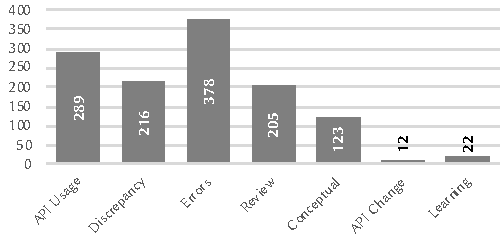
\includegraphics[width=.6\linewidth]{beyerclass}
\caption[Distribution of Stack Overflow question types]{Distribution of \gls{so} question types.}
\label{semotion2020:fig:beyer-classifications}
\end{figure}

\Cref{semotion2020:fig:beyer-classifications} displays the overall distribution of question types from the 1,245 posts classified in~\citep{Cummaudo:2020icse}, when adjusted for majority ruling as per \cref{semotion2020:ssec:method:filtering:classification}. It is evident that developers ask issues predominantly related to \glsac{api} errors when using \glspl{cvs} and, additionally, how they can use the \glsac{api} to implement specific functionality. There are few questions related to version issues or self-learning.

\begin{table}[th]
\caption{Frequency of emotions per question type.}
\label{semotion2020:tab:emotion-freq}
\resizebox{\linewidth}{!}{\begin{tabular}{l|ccccccc|c}
\toprule
\textbf{Question Type}&
\textbf{Fear}&
\textbf{Joy}&
\textbf{Love}&
\textbf{Sadness}&
\textbf{Surprise}&
\textbf{Anger}&
\textbf{No Emotion}&
\textbf{Total}\\
\midrule
\glsac{api} Usage&50&22&34&18&59&13&135&331\\
Discrepancy&38&12&18&7&48&20&108&251\\
Errors&69&34&22&21&48&23&206&423\\
Review&34&16&15&16&42&14&98&235\\
Conceptual&26&10&10&7&21&5&59&138\\
\glsac{api} Change&4&2&2&1&1&1&5&16\\
Learning&3&4&2&0&4&0&11&24\\
\midrule
Total&224&100&103&70&223&76&622&1418\\
\bottomrule
\end{tabular}}
\end{table}

\Cref{semotion2020:tab:emotion-freq} displays the frequency of questions that were classified by EmoTxt when compared to our assignment of question types, while \cref{semotion2020:fig:emotion-dist} presents the emotion data proportionally across each type of question. \textit{No Emotion} was the most prevalent across all question types, which is consistent with the findings of the Collab group during the training of the EmoTxt classifier. Interestingly, \textit{\glsac{api} Change} questions had a distinct distribution of emotions, where 31.25\% of questions had \textit{No Emotion} compared to the average of 42.01\%. This is likely due to the low sample size of \textit{\glsac{api} Change} questions, with only 12 assignments, however the next highest set of emotive questions are found in the second largest sample (\textit{\glsac{api} Usage}, at 59.21\%) and so greater emotion detected is not necessarily proportional to sample size.  Unsurprisingly, \textit{Discrepancy} questions had the highest proportion of the \textit{Anger} emotion, at 7.97\%, compared to the mean of 4.74\%, which is indicative of the frustrations developers face when the \glsac{api} does something unexpected. \textit{Love}, an emotion which we expected least by software developers when encountering issues, was present across the different question types. The two highest emotions, by average, were \textit{Fear} (16.67\%) and \textit{Surprise} (14.90\%), while the two lowest emotions were \textit{Sadness} (4.47\%) and \textit{Anger} (4.74\%). \textit{Joy} and \textit{Love} were roughly the same and fell in between the two proportion ends, with means of 8.96\% and 8.16\%, respectively.

Results from our reliability analysis showed largely poor results. Guidelines of indicative strengths of agreement are provided by~\citet{Landis:1977kv}, where $\kappa \leq 0.000$ is \textit{poor agreement}, $0.000 < \kappa \leq 0.200$ is \textit{slight agreement} and $0.200 < \kappa \leq 0.400$ is \textit{fair agreement}. Our readings were indicative of poor agreement between raters (\cohen{}$=-0.003$) and slight agreement with EmoTxt (\light{}$=0.155$).  The strongest agreements found were for \textit{No Emotion} both between each of our three raters (\light{}$=0.292$) and each rater and EmoTxt (\cohen{}$=0.086$), with fair and slight agreement respectively.

\begin{figure}[tbh]
\centering
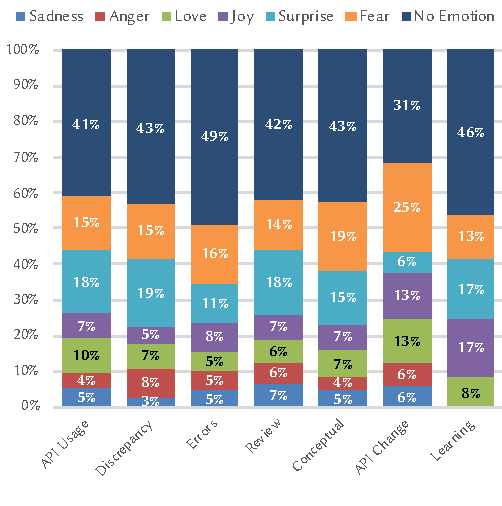
\includegraphics[width=.6\linewidth]{emotionproportion}
\caption[Proportion of emotions per question type]{Proportion of emotions per question type.}
\label{semotion2020:fig:emotion-dist}
\end{figure}

\begin{landscape}
\begin{table*}
\caption[Assigning emotion to Stack Overflow questions]{Sample questions comparing question type to emotion. Questions located at https://stackoverflow.com/q/[ID].}
\label{semotion2020:table:SampleQuestions}
\small
\tablefit{\begin{tabular}{lp{0.71\linewidth}ll}
\toprule
\textbf{ID} &
\textbf{Quote}&
\textbf{Classification}&
\textbf{Emotion}\\
\midrule
53249139&
\textit{``I'm trying to integrate my project with Google Vision \glsac{api}... I'm wondering if there is a way to set the credentials explicitly in code as that is more convenient than setting environment variables in each and every environment we are running our project on... I know for a former client version 1.22 that was possible... but for the new client \glsac{api} I was not able to find the way and documentation doesn't say anything in that regards.''}&
\glsac{api} Usage&
Fear\\
40013910&
\textit{``I want to say something more about Google Vision \glsac{api} Text Detection, maybe any Google Expert here and can read this. As Google announced, their TEXT\_DETECTION was fantastic... But for some of my pics, what happened was really funny... There must be something wrong with the text detection algorithm.''}&
Discrepancy&
Anger\\
50500341&
\textit{``I just started using PYTHON and now i want to run a google vision cloud app on the server but I'm not sure how to start. Any help would be greatly appreciated.''}&
\glsac{api} Usage&
Sadness\\
49466041&
\textit{``I am getting the following error when trying to access my s3 bucket... my hunch is it has something to do with the region...I have given almost all the permissions to the user I can think of.... Also the region for the s3 bucket appears to be in a place that can work with rekognition. What can I do?''}&
Errors&
Surprise\\
55113529&
\textit{''Following a tutorial, doing everything exactly as in the video... Hoping to figure this out as it is a very interesting concept...Thanks for the help... I'm getting this error:...''}&
Errors&
Joy\\
39797164&
\textit{``Seems that the Google Vision \glsac{api} has moved on and the open Sourced version has not....In my experiments this `finds' barcodes much faster than using the processor that the examples show.  Am I missing something somewhere?''}&
\glsac{api} Change&
Love\\
\bottomrule
\end{tabular}}
\end{table*}\end{landscape}


\section{Discussion}\label{semotion2020:sec:discussion}

Our findings from the comparison between the manually annotated \gls{so} posts and the automatic classification revealed substantial discrepancies. \Cref{semotion2020:table:SampleQuestions} provide some sample questions from our data set and the emotion identified by EmoTxt within the text. A subset of questions analysed by our three raters do not indicate the automatic (EmoTxt) emotion, and upon manual inspection of the text after poor results from our reliability analysis, an introspection of the data set sheds some light to the discrepancy. For example, question 55113529 shows no indication of \textit{Joy}, rather the developer is expressing a state of confusion. The phrase \textit{``Thanks for your help''} could be the reason why the miss-classification occurred if words like ``thanks'' were associated with joy. However, in this case, it seems unlikely that the developer is expressing joy as the developer has followed a tutorial but is still encountering an error. Similarly, question 39797164, classified as \textit{Love} and question 50500341, classified as \textit{Sadness} express a state of confusion and the urge to know more about the product; upon inspecting the entire question in context, it is difficult to consistently agree with the emotions as determined by EmoTxt, and further exploration into the behaviour and limitations of the model is necessary.

Our results indicate further work is needed to refine the \gls{ml} classifiers that mine emotions in the \gls{so} context. The question that arises is whether the classification model is truly reflective of real-world emotions expressed by software developers. As highlighted by~\citet{curumsing2017}, the divergence of opinions with regards to the emotion classification model proposed by theorists raises doubts to the foundations of basic emotions. Most of the studies conducted in the area of emotion mining from text is based on an existing general purpose emotion framework from psychology~\citep{Ondrej:2016, ortu2016, novielli2018}---none of which are tuned for software engineering domain. In our our study, we note the emotions expressed by software developers within \gls{so} posts are quite narrow and specific. In particular, emotions such as frustration and confusion would be more appropriate over love and joy. 
%To the best of our knowledge, no such classification exist in the literature. Studies such as ~\citep{wrobel2013} that list of emotions expressed by software developers and our findings can potentially be combined to create an emotion set better aligned to online questions.

\section{Implications}\label{semotion2020:sec:implications}

Based on our observations during the manual classification of \gls{so} posts and related work in the field~\citep{wrobel2013}, we propose a new taxonomy of emotions which is reflective of what software developers experience when encountering coding issues. We propose the following set of five emotions: 
(i) \textit{Confusion}, an inability to understand something, e.g., \textit{``why is the code not functioning?''} or \textit{``where is the error?''};
(ii) \textit{Frustration}, annoyance resulting from the inability to change or achieve something, e.g., \textit{``I don't understand why this code is not working.''};
(iii) \textit{Curiosity}, an urge to learn more about the tool, e.g., \textit{``I am looking for a way to do this...''};
(iv) \textit{Contentedness}, where developers are satisfied with the current situation however there may be a small issue, e.g., \textit{``It works pretty well, but...''}; and,
(v) \textit{Optimism}, hopeful that a solution can be found, e.g., \textit{``I hope you can see what I'm doing wrong.''}.

%Our proposed taxonomy was tested on the same set of 25 randomly selected \gls{so} posts by the same three testers. The testers agreed that the new taxonomy is more reflective of what software developers express within \gls{so} posts and identified \textit{confusion} and \textit{curiosity} as being the highly rated emotions.

\section{Threats to Validity}\label{semotion2020:sec:threats}

\subsection{Internal Validity} 
The \textit{\glsac{api} Change} and \textit{Learning} question types were few in sample size (only 12 and 22 questions, respectively). The emotion  proportion distribution of these question types are  quite different to the others.  Given the low number of questions, the sample is too small to make confident assessments. Furthermore, our assignment of~\citeauthor{Beyer:2018fm}'s question type taxonomy was single-label; a multi-labelled approach may work better, however analysis of results would become more complex. A multi-labelled approach would be indicative for future work. Lastly, the study would be greatly improved with a reliability analysis of our proposed taxonomy; while we did resolve using majority voting (\cref{semotion2020:ssec:manual}), no inter-rater reliability has been performed for this study. We plan to conduct reliability analysis, expand the number of raters, and increase the 25 question sample size in our future work for a more thorough analysis of our proposed taxonomy. 

\subsection{External Validity}
EmoTxt was trained on questions, answers and comments, however our data set contained questions only. It is likely that our results may differ if we included other discussion items, however we wished to understand the emotion within developers' \textit{questions} and classify the question based on the question classification framework by~\citet{Beyer:2018fm}. Moreover, this study has only assessed frustrations within the context of a concrete domain of \glspl{cvs}. The generalisability of this study to other \glspl{iws}, such as natural language processing services, or conventional web services, may be different. Furthermore, we only assessed four popular \glspl{cvs}; expanding the data set to include more services, including non-English ones, would be insightful. We leave this to future work.

\subsection{Construct Validity}
Some posts extracted from \gls{so} were false positives. Whilst flagged for removal (\cref{semotion2020:ssec:method:filtering:automated-manual-filtering}), we cannot guarantee that all false positives were removed. Furthermore, \gls{so} is known to have questions that are either poorly worded or poorly detailed, and developers sometimes ask questions without doing any preliminary investigation. This often results in down-voted questions. We did not remove such questions from our data set, which may influence the measurement of our results.


\section{Conclusions}\label{semotion2020:sec:conclusion}

In this paper we analysed \gls{so} posts for emotions using an automated tool and cross-checked it manually. We found that the distribution of emotion differs across the taxonomy of issues, and that the current emotion model typically used in recent works is not appropriate for emotions expressed within \gls{so} questions. Consistent with prior work~\citep{lin2018sentiment}, our results demonstrate that machine learning classifiers for emotion are insufficient; human assessment is required.

Future work would include validating our proposed taxonomy of emotions through (1) a survey with software developers to identify the validity of the emotions present in the taxonomy; (2) manually classifying \gls{so} posts using the proposed emotion classification model to study the distribution of \gls{so} posts under each taxonomy of errors; and (3) extend the work to other communication channels used by software developers. 